\section{Discussion}

\ACL{sorn}s are a promising approach in modeling brain processes. \acs{sorn} extends randomly initialized reservoir networks with binary threshold neurons by using three biologically motivated plasticity mechanisms. It has already been shown that this self-organizing network outperforms static reservoir networks and is able to reproduce experimental findings, shown in section \ref{sec:prop-sorn}. \textcite{lazar2009sorn} stated that many basic mechanisms, like plasticity mechanisms, are more and more researched. Even though those mechanisms still lack a deep understanding, it is highly interesting how they work together in a balanced system. The hope is to get a deeper understanding of basic processes of dynamic non-linear systems, like the brain. 

Since the number of neurons in the network is relatively small, in a scale of hundreds, the applications are limited to sensory or short-term processes. Indeed, when \acl{stdp} was active in the testing phase, the network tends to forget the stored information by time. It should be possible to build larger networks using \acs{sorn}, for example in combination with cell assemblies. At present, cell assemblies are often build with static reservoir networks, but first dynamic approaches already exist \parencite{dasgupta2015self, tetzlaff2015use}.

However, this thesis focuses on a small sized network and its properties. The combination of the plasticity rules led to the interesting finding, that different input patterns highly influence how well the network is able to store and reproduce this input. Furthermore, it was hypothesized that \acl{ip} plays in important role for those results.

\subsection{Perspectives on SORN}

There are severals mathematical perspectives to interpret \acs{sorn}. Three variants could be collected.

\begin{itemize}
\item Trajectory in high dimensional space: The (spontaneous) activity in the network, with its $N^E$ neurons, can be seen as a trajectory in an $N^E$-dimensional space. This perspective has similarities with kernels. The input is transformed in a high dimensional time-dependent feature space, which was already discussed in section \ref{sec:res-net}.
\item \acl{mcmc} sampling: If the time-dependent input pattern is modeled with a Markov chain, the network learns from Markov chain samples. Furthermore, in testing phase, the network reproduces those samples.
\item Statistical estimator: Again, if \acs{sorn} is trained, using a distribution for the input neurons, the network can be seen as an estimator for this distribution. The parameters of the network determine the quality of the estimator. If the underlying Markov chain is unknown, it can be estimated by the (spontaneous) activity patterns of the network.
\end{itemize}

Regarding the sampling perspective, the samples from the Markov chain could be biased while training. According to the law of large numbers, after a long time the average converges to the Markov distribution. But in finite time steps, it is possible to have large runaways. Therefore, it is not guaranteed that the network was trained with a perfect Markov chain. This effect could be stronger in those networks, where some states are repeated very often. To put it in other words, in testing phase, the network does not reproduce the Markov chain, it reproduces the \emph{samples} from the training phases, which were samples from the Markov chain. However, since the results are averaged over $\Nsim$ runs and the standard error was calculated, this influence is assessable.

\subsection{Reverse learning effect}

\textcite{hartmann2015s} applied different probabilities to $8$ input states. States $A$, $B$, $C$ and $D$ occurred with a probability between $\frac{0.1}{4} = 0.025$ and $\frac{0.9}{4} = 0.225$ for each state. In contrary, states $E$, $F$, $G$ and $H$ were active with the reverse probability between $\frac{0.9}{4}$ and $\frac{0.1}{4}$. The probabilities were changed in steps of $0.1$. In figure \ref{fig:reverse-effect} the results are shown. Between $0.2$ and $0.8$, the network was able to reproduce the initial probabilities with a small amount of over representation. But at $0.1$/$0.9$, the effect was reversed and the variance increased. \textcite{hartmann2015s} argued that this effect is due to `pathological network dynamics', while a specific explanation was missing. It is suggested that the \acs{ip}-hypothesis is able to explain the reverse effect. Probably, the states were changing fast enough and avoiding distorting spontaneous activity in the range between $0.2$ and $0.8$. After that, it is likely that the threshold becomes smaller than zero, before the state is activated again according to the rule.

\begin{figure}[!t]
    \centering
    \begin{subfigure}[t]{0.48\textwidth}
    	\centering
        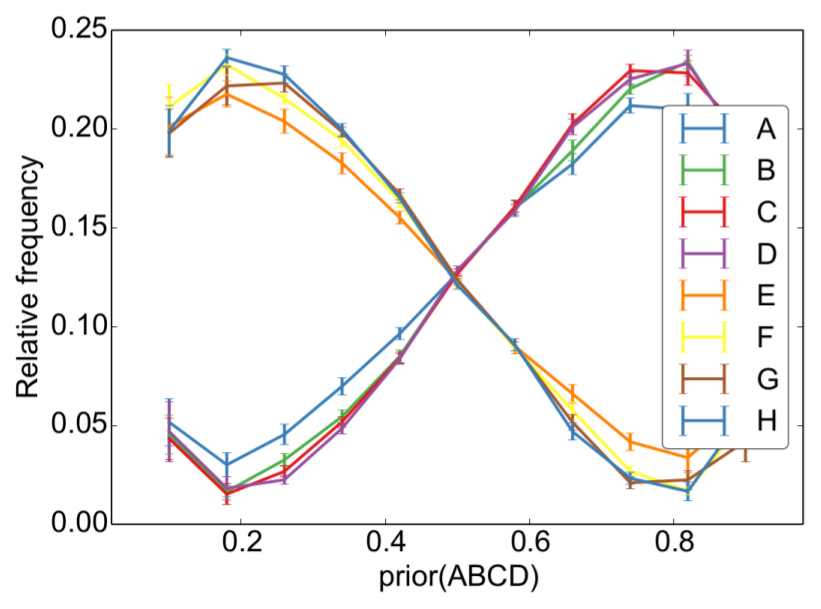
\includegraphics[width=\textwidth]{discussion/reverse-effect}
        \caption{States $A$, $B$, $C$ \& $D$ and $E$, $F$, $G$ \& $H$  were learned with probabilities between $0.1$ and $0.9$. At the extreme points, a reverse effect in the representation was observed \parencite[figure 4c]{hartmann2015s}. It can possibly be explained with \acl{ip}.}
        \label{fig:reverse-effect}
    \end{subfigure}
    \hfill
    \begin{subfigure}[t]{0.48\textwidth}
    	\centering
        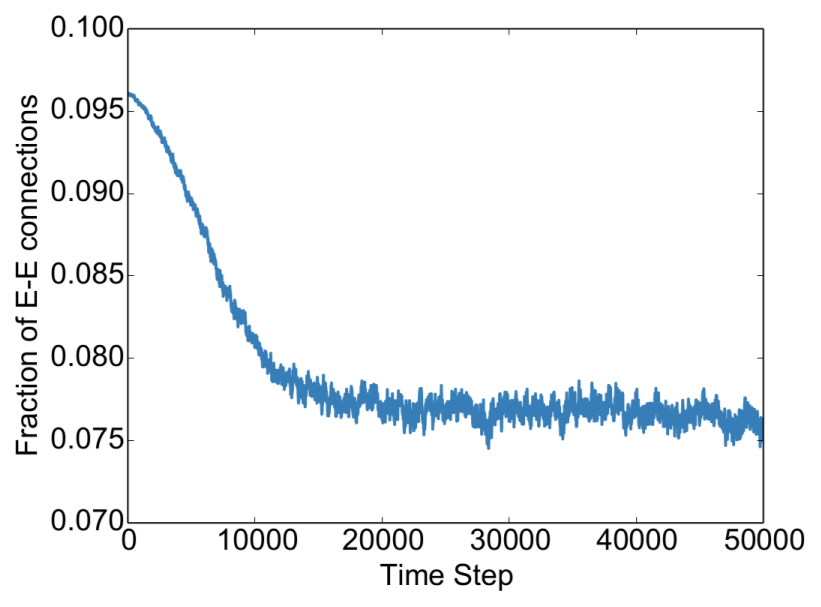
\includegraphics[width=\textwidth]{discussion/ex-to-ex}
        \caption{The fraction of excitatory-to-excitatory connections, where $w_{ij} > 0$ during plastic training, stabilizes after about $20,000$ steps \parencite[figure 1d]{hartmann2015s}. It is assumed to correspond to the error decay in the first $20,000$ steps of training.}
        \label{fig:ex-to-ex}
    \end{subfigure}
    \caption[Reverse learning effect and fraction of excitatory-to-excitatory connections]{Reverse learning effect and fraction of excitatory-to-excitatory connections from \textcite{hartmann2015s}.}
    \label{fig:hartmann-figs}
\end{figure}

\subsection{Biological plausibility}

The question arises if the differences in the learning performance are due to \acs{sorn} alone or if there are indications that this behavior can also be observed in experiments where responses from mammal brains are recorded. In psychology, an experimental design, called \emph{oddball paradigm}, is often used for recording the neural behavior of time-dependent stimulus patterns. It consists of a \emph{standard} stimulus, which is repeated very often, and a \emph{deviant}, which breaks the previous stimuli. If the electrophysiological or magnetophysiological activity of the brain is recorded, a deviant elicits an \acfi{erp} or more specific a \acfi{mmn}. The electro- or magnetophysiological activity differs significantly from normal activity when a deviant stimulus is presented \parencite{naatanen1978early}.

The processes, underlying the \acs{mmn} mechanism, is assumed to be pre-attentive and on a sensory memory level \parencite{tiitinen1994attentive}. While the \acs{mmn} was obtained with simple stimulus rules, \textcite{paavilainen2007preattentive} and \textcite{bendixen2008rapid} were able to show that also more complex stimulus rules can be learned and detected by the brain. Such a rule is shown in figure \ref{fig:oddball-rule}. The learning of those complex rules is not accessible to attentive processing, which emphasizes that the detection mechanisms is connected to processing on sensory level. As already stated above, \acs{sorn} has also characteristics of a sensory or short-term memory. Thus, a parallel between those experiments with humans and the simulation can be drawn. Furthermore, in a more broad perspective, the difference between standard and deviant stimuli can be seen as stimuli which are more probable or less probable, respectively. The input patterns can therefore be modeled as Markov chains, which was done by \textcite{mill2011neurocomputational}. They found that the way the deviants, or less probable states, are represented in the network, highly depends on the parameters of the system, which was also found in this thesis.

\begin{figure}[!t]
	\centering
	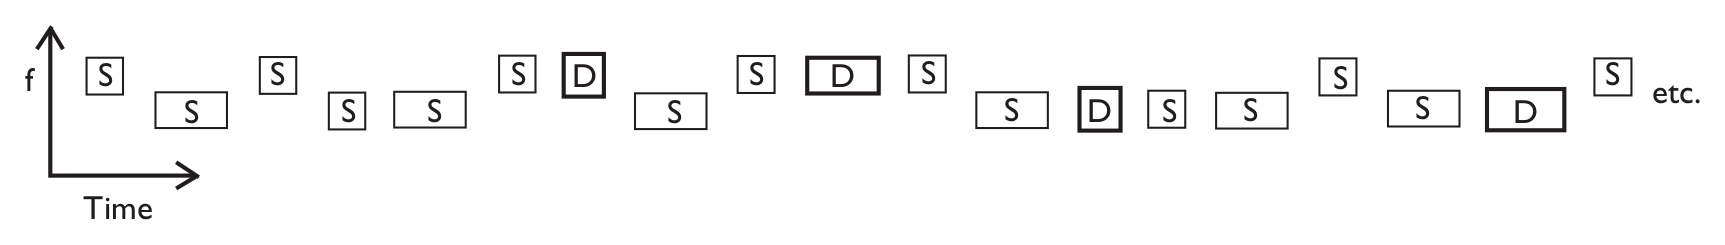
\includegraphics[width=\textwidth]{discussion/oddball-rule}
	\caption[Complex rule used in oddball paradigm]{Complex rule with auditory stimuli used in oddball paradigm \parencite[figure 1]{paavilainen2007preattentive}. Long tones are followed by high tones (high frequency $f$) and short tones are followed by low tones. $S$ indicates a standard stimuli, fitting to the rules, $D$ indicates a deviant, breaking the rule.}
	\label{fig:oddball-rule}
\end{figure}

To the best of the authors knowledge, there are no experimental findings which either clearly supports the exact findings, nor rejects it. However, there is a lot of evidence that less probable stimuli are processed in a special way. In future research, it would be an interesting approach to use the oddball paradigm to train different stimuli patterns to the brain using Markov chains. Results from such an experiment would probably reveal if the effect from the simulation also appears in natural networks.

Another biological relation can be found regarding the plastic training. In the results section, figure \ref{fig:mc1-training} shows that the network needs about $20,000$ steps of plastic training, until the performance becomes stable and further training does not influence the performance any more. Interestingly, there seems to be a parallel to the observation that the fraction of excitatory-to-excitatory connections stabilizes after some time. The fraction designates how many weights stay with a weight of $w_{ij} > 0$ during plasticity training. Many weights, which are not necessary for the input pattern, decay to zero or close to zero, due to \acs{stdp}. This effect is known to occur in natural networks \parencite{yasumatsu2008principles}. In figure \ref{fig:ex-to-ex} a plot from \textcite{hartmann2015s} is shown. It takes about $20,000$ steps of training until the stable fraction was reached. This corresponds to the training time of the network and possibly explains the ceiling effect of training steps. As long as non-necessary connections exist, the input pattern cannot be reproduced very well. A ceiling is reached, when the fraction stabilizes. At that point no further increase in performance should be possible.

As already mentioned in section \ref{sec:prop-sorn}, \textcite{zheng2013network} extended a \acs{sorn} with structural plasticity. After every step, with a low probability, new connections were established. With this mechanism it should be possible to extend the learning phase slightly. It could possibly also reduce the effects due to the \acs{ip} mechanism. Furthermore, while initializing the connections, a stochastic component to the connectivity of every neuron could be added. The connectivity $\lambda^W$ would stay the same as before, but it would become the mean connectivity per neuron instead of a fixed connectivity per neuron. A stochastic component with a specific distribution could add variation to every neuron.

\subsection{Markov chains}

Directly connected to the former suggestion, it would be interesting to apply multi-state Markov chains. Currently, only one state is active at a specific point in time. This holds for the plastic and no-plastic training as well as for the testing phase, where only one state is classified for each step. But in more complex rules, a stimulus can have more than one property. For example in the experiments from \textcite{paavilainen2007preattentive} and \textcite{bendixen2008rapid}, the auditive stimuli were different in their pitch \emph{and} in their length. Therefore, it would be interesting to define an input cluster for low and high tones as well as an input cluster for short and long tones. At a specific point in time always two clusters are active: low/short, low/long, hight/short, hight/long. Using such a Markov chain would enable the network to possibly reproduce the experimental findings.

According to the \acs{ip}-hypothesis, also the number of states $n$ of the Markov chain should be important. In the present thesis, only Markov chains with $n=4$ states were tested. But it can be predicted that if the number of states increase, the performance should decrease, due to \acl{ip}. If only one state is active at a time and many states are available, it takes possibly a long time until the current state will be activated again. Therefore, spontaneous activity will activate neurons in different clusters of the network and the classification will be at least more ambiguous. Markov chains with $n > 4$ should be tested in combination with $k > 1$ in the $k$-nearest neighbor classification algorithm (see below) in order to observe if the ambiguous behavior happens as predicted or not.

Another aspect is the prediction problem. The stationary distribution was only appropriate in some cases. A better predictor could possibly be derived from the transition matrix directly, since it contains much more information than the stationary distribution. A clustering algorithm for Markov chains, as it was developed by \textcite{van2001graph}, could possibly be an interesting candidate. If some states have a high probability to each other, but a low probability to the others, the chain ends up in lower performance, due to \acl{ip}. This structure could be reflected by a clustering algorithm.

\subsection{Classification}

In the current network simulation, the classification was done with an algorithm which is similar to a $k$-nearest neighbor algorithm with $k = 1$. The distance between an activity pattern in the testing phase and every activity patterns in the no-plastic training phase was calculated. The activity pattern from the no-plastic training phase with minimum distance was used for classification. An extension to this algorithm could be a $k$-nearest neighbor algorithm with $k > 1$, such that $k$ closest activity patterns from the no-plastic training phase are taken for classification. The majority of appearing states would be the classified state. This has two advantages:

\begin{itemize}
\item It is easier to evaluate ambiguous classifications. In appendix \ref{sec:appendix:hamming} the classification method was evaluated. While the hamming threshold criterion was able to exclude ambiguous states, it is not able to classify which state is the second closest. With $k > 1$ it is very easy to classify specific input patterns as ambiguous and to get information about which states are involved in that case.
\item It allows classification of two or more states. If a multi-state Markov chain would be used, it is necessary to classify which states are currently active. A classification with $k = 1$ only considers one activity pattern. Therefore, $k>1$ is necessarily needed to classify multiple states. To be precise, $k$ needs to be at least as high as the number of simultaneously active states.
\end{itemize}

\subsection{IP mechanism}
\label{sec:discuss-ip}

\begin{figure}[!b]
	\centering
	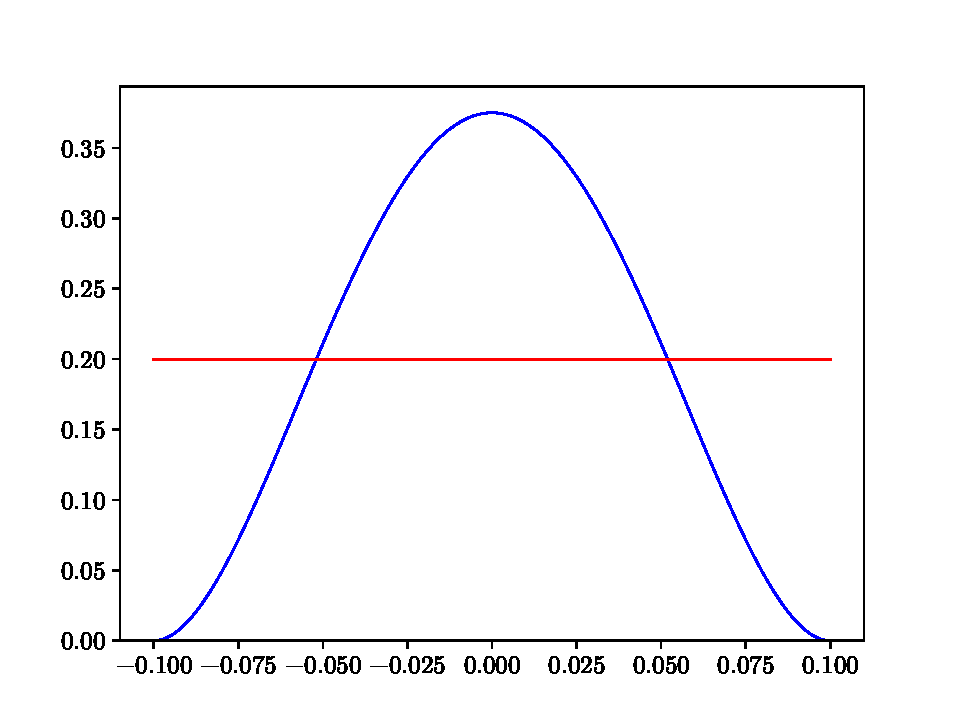
\includegraphics[width=0.75\textwidth]{discussion/beta}
	\caption[Beta distribution]{Beta distribution which can be used for $\varepsilon_i^\IP$, instead of a uniform distribution. The blue line shows the probability density function of a Beta distribution, where $\alpha = \beta = 3$. The distribution is centralized and divided by a scaling factor of $5$. The red line is the probability density function of a uniform distribution with $a = -0.01$ and $b = 0.01$, as it was already used in \textcite{hartmann2015s} and in this thesis. The same results from a Beta distribution with $\alpha = \beta = 1$, which is centralized and divided by $5$ again.}
	\label{fig:beta-dist}
\end{figure}

Regarding the \acs{ip} mechanism, the distribution for the target rate range, introduced in equation \eqref{eq:hip-ind}, could be modified. For stability reasons the target rate $H^\IP$ is not fixed \parencite{hartmann2015s}. A term $\varepsilon_i^\IP$ was added, introduced in section \ref{sec:ip-mod}, which is uniformly distributed with $\varepsilon_i^\IP \sim \text{Uni}[a,b] = \text{Uni}[-\sigma^\IP,+\sigma^\IP] = \text{Uni}[-0.01,0.01]$. $\sigma^\IP$ was already systematically changed, shown in figure \ref{fig:hip-range}. Since it was not possible to reproduce the previous results, perhaps another approach could be interesting. Possibly, if $\varepsilon_i^\IP$ is sampled from another distribution, the results would change. A uniformly distributed $\varepsilon_i^\IP$ has the advantage that it has no infinite tails. Therefore, there are no outliers or, in other words, the range of the outliers can easily be controlled. But on the other hand, the uniform distribution does not concentrate its probability mass around the expectation value, like a normal distribution would do. An interesting candidate would be a Beta distribution which can be centralized and scaled to fit to the requirements. It has the advantage, that is has finite tails and a concentration around the expectation value if the parameters are chosen in an appropriate way with $\alpha = \beta > 1$. Note that the uniform distribution is just a special case of the Beta distribution with $\alpha = \beta = 1$. An example for a suitable Beta distribution is shown in figure \ref{fig:beta-dist}. It is compared to a uniform distribution.

Finally, the variation of the target rate $\bar H^\IP$ in section \ref{sec:ip-hyp} lacks of the activity interaction. The higher $\bar H^\IP$, the higher is the activity in the network and vice versa. To keep the overall activity at a specific level, noise could be implemented. Additional activation can be sampled by a normal distribution with zero expectation value and some variance for every neuron. After every step, this additional activation is added to the actual activation of all neurons. The network would loose its deterministic character in favor of a stable average firing rate. The tricky task is to find a variance for that distribution, which would be able to provide the desired activity level.

\subsection{Conclusion}

\acs{sorn} seems to be an attractive approach for neural simulations, since it allows to research on dynamic behavior of networks. In previous work, simulations showed that \acs{sorn} performs very well and is able to reproduce biological findings \parencite{lazar2009sorn, zheng2013network,  aswolinskiy2015rm, hartmann2015s}. The input of those simulations was chosen in relation to specific biological experiments. In the present approach the input patterns were generalized using \acl{mcmc}. The network was trained with samples from systematically chosen Markov chains. The performance was measured with a \acl{mse} between the initially chosen transition matrix from the Markov chain and the learned transition matrix, calculated by the occurring pattern of states in the network.

It was shown that the performance of the network depends on the chosen Markov chain. If the states of the Markov chain are very regular, which means that the probability between the states is relatively equal, the performance was very high, significantly higher than the performance of static reservoir networks. On the other hand, if the states are irregular and the probability of some states differ a lot from others, the performance is low. It converges to the performance of a static reservoir network with increasing irregularity.

In order to find an explanation for this behavior, parameters and properties of the network were tested, such as the size of the network, the training time and the classification mechanism. It was finally suggested that the \acl{ip} plays an important role for the observed performance differences. The so called \acs{ip}-hypothesis suggests that those states which were not active for a longer time will spontaneously be active, due to the decreasing threshold of the \acs{ip} rule. This hypothesis was able to explain the behavior of many different series of Markov chains. Furthermore, when the target rate, the main parameter of the \acl{ip}, was decreased, the effect was reduced. That clearly shows the influence of the \acs{ip} mechanism on the observed differences between the models. Effects from other parameters could be excluded, like the target rate range, the \acs{ip} learning rate and the connectivity of the network.

Further improvements of the network and future research was discussed. It was suggested to improve the \acl{ip} by choosing another distribution for the target rate range. To validate the influence of the target rate, noise could be included when varying the target rate parameter, in order to keep the activity level stable. Furthermore, the classification mechanism could be extended to a $k$-nearest neighbor algorithm with $k>1$. Finally, in order to be able to reproduce more biological findings, a multi state Markov chain could be applied to \acs{sorn}.

In sum, the Markov chain approach unveiled an interesting behavior of the network, showing that \acs{sorn} does not outperform static reservoir networks in every case. The network behavior is not necessarily independent from its time-dependent input pattern. Further investigations showed that the \acl{ip} has a special role in the network regarding the observed effects. Finally it remains to be tested if indications for the present findings can be found by biological experiments.



%\acs{sorn} seems to be an attractive approach for neural simulations, since it allows to research on dynamic behavior of networks. The input, which is used to train a network, was generalized using Markov chains and the results have shown that a network behavior is not necessarily independent from its time-dependent input pattern, where \acs{ip} is suggested to be responsible for. If a specific event in a stimulus pattern with many possible events is highly probable, intuitively, every deviation from this likely event would be perceived as an `interesting' or `important' information. Otherwise, if all possible events in this stimulus pattern are highly regular, it would not take our attention too much, except we want to. If we just think of listening to a harmonic piece of music from a vinyl record, which is interrupted by a scratch from time to time, the single scratches would get our attention, unless the scratches are very often and more or less regular. In many experiments, like the oddball experiments introduced above, deviants could just be understood as very unlikely events and it was shown in several experiments that the brain reacts more intense to those unlikely events \parencite{paavilainen2007preattentive, bendixen2008rapid, bunzeck2006absolute}. Since there is a link between findings from oddball paradigm with deviants and findings in this thesis regarding learning performances with unlikely events, \acs{ip} is probably strongly connected to pre-attentive learning. This type of plasticity could be a low level mechanism which helps to implicitly process regular information. The processing of highly irregular evens is left for other mechanisms, possibly on a higher level. From an evolutionary perspective it makes sense to process regular information on a lower level rather than unlikely and possibly `dangerous' information. The latter needs our attention to be evaluated on a higher level, in order to take decisions and regulate emotions. According to this theory, \acs{ip} allows free capacity on higher levels for less probable and perhaps more important events, because low level mechanisms like \acs{ip} already perform easily predictable stimuli implicitly.




